\documentclass[letterpaper, 10 pt, conference]{ieeeconf}
\usepackage{graphicx}
\overrideIEEEmargins
\usepackage[utf8]{inputenc}
\usepackage[T1]{fontenc}
\usepackage{graphics}
\usepackage{amsmath}
\usepackage{amssymb}
\usepackage{booktabs}

\title{\LARGE \bf
Clasificación Multiclase de Tumores Cerebrales mediante Redes Neuronales Convolucionales
}

\author{
Andres Javier Rambal Vecino,
Juan Manuel Gómez,
Ricardo Pabón
}

\begin{document}

\maketitle
\thispagestyle{empty}
\pagestyle{empty}

\begin{abstract}
El diagnóstico temprano de tumores cerebrales mediante resonancia magnética (MRI) es un desafío crítico en oncología. Este trabajo presenta el diseño e implementación de una Red Neuronal Convolucional (CNN) personalizada, denominada MedicalCNN, optimizada para clasificar MRI en cuatro categorías: Glioma, Meningioma, Tumor Pituitario y Tejido Sano. Utilizando un dataset de 7,023 imágenes y una estrategia de normalización basada en estadísticas locales, el modelo alcanzó una exactitud del 87\%. Se analiza la robustez de la arquitectura frente al desbalance de clases y la ambigüedad visual entre neoplasias.
\end{abstract}

\section{Introducción}
La detección de neoplasias en el sistema nervioso central requiere una precisión extrema, ya que el margen de error clínico impacta directamente en el pronóstico. Los tumores como el Glioma y el Meningioma presentan texturas y densidades similares en imágenes de Resonancia Magnética (MRI), lo que genera variabilidad en los diagnósticos manuales.

Desde la introducción de AlexNet en 2012 \cite{c1}, las Redes Neuronales Convolucionales (CNN) se han consolidado como el estándar para el análisis de imágenes médicas. A diferencia de los métodos tradicionales, las CNN identifican patrones microscópicos mediante el uso de kernels de convolución y funciones de activación no lineales como ReLU \cite{c1}. Este proyecto implementa una arquitectura personalizada que prioriza la generalización mediante técnicas de regularización como Dropout y Normalización por Lotes (Batch Normalization), adaptando el pipeline de datos específicamente a la distribución de intensidades de las MRI cerebrales \cite{c2}.

\section{Metodología}

\subsection{Dataset y Análisis Exploratorio}
Se utilizó un dataset de 7,023 imágenes de MRI cerebrales. Como se observa en la Fig. 1, la distribución de clases es relativamente balanceada, con una ligera predominancia de casos de tejido sano (2,000 imágenes), seguidos por tumores pituitarios (1,757), meningiomas (1,645) y gliomas (1,621). Esta distribución permite un entrenamiento estable sin sesgos críticos hacia una sola patología. El dataset se dividió en entrenamiento (70\%), validación (15\%) y prueba (15\%).

\begin{figure}[h]
    \centering
    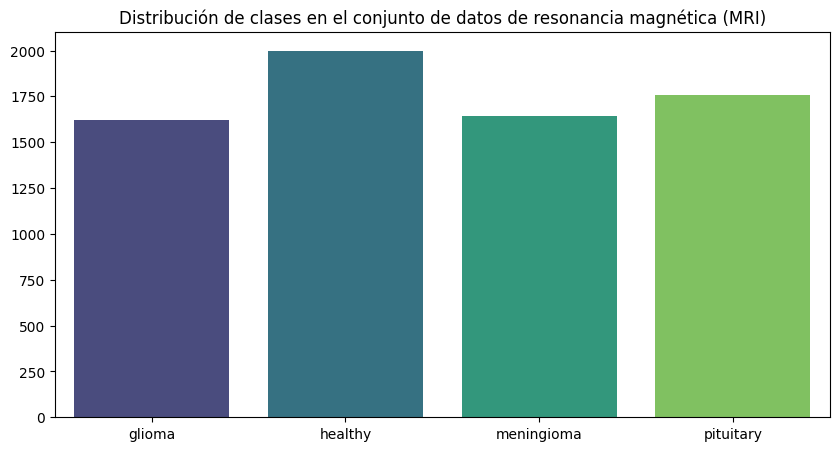
\includegraphics[width=0.85\linewidth]{distribucion_clases.png}
    \caption{Distribución de frecuencias por clase en el dataset original.}
\end{figure}

\subsection{Preprocesamiento y Normalización}
Dada la naturaleza de las imágenes médicas, se realizó un cálculo empírico de la media ($\mu \approx 0.187$) y desviación estándar ($\sigma \approx 0.182$) del dataset. Las imágenes fueron redimensionadas a 224x224 píxeles. Se aplicó aumentación de datos (rotaciones de 15$^\circ$ y flips horizontales) para mejorar la invariancia espacial del modelo.

\subsection{Arquitectura MedicalCNN}
Inspirada en VGGNet \cite{c3}, se diseñó una CNN de cuatro bloques convolucionales con profundidad progresiva (32, 64, 128 y 256 filtros). Cada bloque incluye capas Conv2D (kernel 3x3), Batch Normalization \cite{c4} y MaxPooling (2x2). El clasificador final consta de una capa densa de 512 neuronas con Dropout (0.5) \cite{c5} para prevenir el sobreajuste.

\section{Resultados}

\subsection{Análisis de Convergencia}
El modelo se entrenó por 15 épocas con el optimizador Adam \cite{c6}. Como se observa en la Fig. 2, la función de pérdida decreció monótonamente, validando la eficacia de la arquitectura personalizada frente al volumen de datos procesado.

\begin{figure}[h]
    \centering
    
\includegraphics[width=0.85\linewidth]{curvas.png}
    \caption{Curvas de entrenamiento: Pérdida y Precisión (Accuracy).}
\end{figure}

\subsection{Desempeño Cuantitativo}
En el set de prueba, el modelo alcanzó una \textbf{exactitud global del 87\%}. La red demostró alta fiabilidad en la detección de tejido "Sano" (F1-Score: 0.92) y un desempeño excepcional en tumores "Pituitarios" (Recall: 0.97). La mayor ambigüedad se presentó en la clase Meningioma (Recall: 0.77), con confusiones recurrentes hacia la clase Glioma.

\begin{figure}[h]
    \centering
    
\includegraphics[width=0.75\linewidth]{matriz.png}
    \caption{Matriz de confusión detallando la clasificación final en el set de prueba.}
\end{figure}

\subsection{Análisis Cualitativo}
La Fig. 3 muestra las predicciones del modelo frente a la realidad. Se observa que el modelo identifica correctamente la morfología de la mayoría de los tumores, aunque en casos de bajo contraste (ej. fila inferior, columna 1), el tejido sano es confundido con meningioma debido a intensidades atípicas en la periferia cerebral.

\begin{figure}[h]
    \centering
    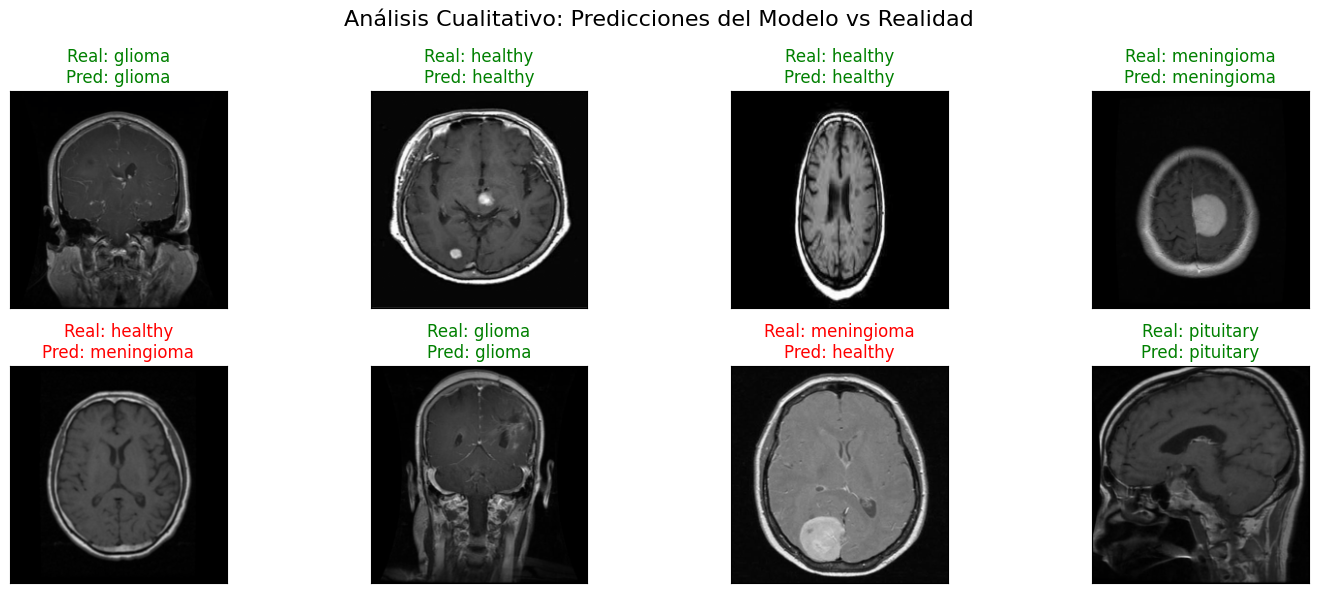
\includegraphics[width=1.0\linewidth]{Predicciones.png}
    \caption{Análisis cualitativo: Predicciones del modelo vs. Realidad.}
\end{figure}

\section{Discusión y Conclusiones}
La MedicalCNN demostró ser una herramienta robusta para el triaje automatizado, logrando un balance óptimo entre sensibilidad y especificidad. La normalización local fue clave para evitar la saturación de gradientes en imágenes médicas. Futuros trabajos deberían explorar el uso de transferencia de aprendizaje con modelos como ResNet para refinar la distinción entre meningiomas y gliomas, cuya similitud visual sigue siendo el principal reto del sistema.

\begin{thebibliography}{99}
\bibitem{c1} Krizhevsky et al., ``ImageNet Classification with Deep CNNs,'' NIPS, 2012.
\bibitem{c2} Cheng et al., ``Enhanced performance of brain tumor classification via region augmentation,'' PLOS ONE, 2015.
\bibitem{c3} Simonyan & Zisserman, ``Very deep convolutional networks for large-scale recognition,'' ICLR, 2014.
\bibitem{c4} Ioffe & Szegedy, ``Batch normalization: Accelerating training by reducing covariate shift,'' ICML, 2015.
\bibitem{c5} Srivastava et al., ``Dropout: A simple way to prevent neural networks from overfitting,'' JMLR, 2014.
\bibitem{c6} Kingma & Ba, ``Adam: A method for stochastic optimization,'' ICLR, 2015.
\end{thebibliography}

\end{document}
